\documentclass[12pt,a4paper,bibliography=totocnumbered,listof=totocnumbered]{scrartcl}
\usepackage[ngerman]{babel}
\usepackage[utf8]{inputenc}
\usepackage{amsmath}
\usepackage{amsfonts}
\usepackage{amssymb}
\usepackage{graphicx}
\usepackage{fancyhdr}
\usepackage{tabularx}
\usepackage{geometry}
\usepackage{setspace}
\usepackage[right]{eurosym}
\usepackage{subfig}
\usepackage{floatflt}
\usepackage[usenames,dvipsnames]{color}
\usepackage{colortbl}
\usepackage{paralist}
\usepackage{array}
\usepackage{titlesec}
\usepackage{parskip}
\usepackage[right]{eurosym}
\usepackage[subfigure,titles]{tocloft}
\usepackage[pdfpagelabels=true]{hyperref}
\usepackage{amsthm}
\usepackage{listings}
\usepackage{mdframed}
\usepackage{pdfpages}
\usepackage{breqn}
\usepackage[german]{algorithm2e}
\usepackage{url}
\usepackage{tikz}
\usepackage{pgfplotstable}
\usepackage{lineno}

\nonstopmode

%FIXME: Ist das besser?
\newtheoremstyle{hagerup}%
  {3pt}%
  {3pt}%
  {\itshape}%
  {}%
  {}%
  {:}%
  {.5em}%
  {\textbf{\thmname{#1}\thmnumber{ #2}}\thmnote{ -- #3}}

\newtheorem{claim}{Behauptung}
\newtheorem{theorem}{Satz}
\newtheorem{lemma}{Lemma}
\newtheorem{corollary}{Korollar}

\theoremstyle{hagerup}
\newtheorem{definition}{Definition}

\geometry{a4paper, top=27mm, left=30mm, right=20mm, bottom=35mm, headsep=10mm, footskip=12mm}

\pgfplotstableread{img/gausssteps/default_0.dat}\matrixdefaulta
\pgfplotstableread{img/gausssteps/default_1.dat}\matrixdefaultb
\pgfplotstableread{img/gausssteps/default_2.dat}\matrixdefaultc
\pgfplotstableread{img/gausssteps/default_3.dat}\matrixdefaultd
\pgfplotstableread{img/gausssteps/default_4.dat}\matrixdefaulte
\pgfplotstableread{img/gausssteps/default_5.dat}\matrixdefaultf
\pgfplotstableread{img/gausssteps/default_6.dat}\matrixdefaultg
\pgfplotstableread{img/gausssteps/default_7.dat}\matrixdefaulth

\pgfplotstableread{img/gausssteps/optimized_0.dat}\matrixpeoa
\pgfplotstableread{img/gausssteps/optimized_1.dat}\matrixpeob
\pgfplotstableread{img/gausssteps/optimized_2.dat}\matrixpeoc
\pgfplotstableread{img/gausssteps/optimized_3.dat}\matrixpeod
\pgfplotstableread{img/gausssteps/optimized_4.dat}\matrixpeoe
\pgfplotstableread{img/gausssteps/optimized_5.dat}\matrixpeof
\pgfplotstableread{img/gausssteps/optimized_6.dat}\matrixpeog
\pgfplotstableread{img/gausssteps/optimized_7.dat}\matrixpeoh

\definecolor{light-gray}{gray}{0.90}

\newcommand{\spymatrix}[1]{\resizebox{\columnwidth / 4}{!}{
		\begin{tikzpicture}
			\foreach \i in {0,...,7}{
					\foreach \j in {0,...,7}{
							\pgfplotstablegetelem{\i}{\j}\of#1
							\ifnum\pgfplotsretval=0
								\node[circle, minimum size=.5pt, inner sep=0pt, fill=light-gray] at (\j pt,-\i pt) {};
							\else
								\ifnum\pgfplotsretval=1
									\node[circle, minimum size=.5pt, inner sep=0pt, fill=red] at (\j pt,-\i pt) {};
								\else
									\node[circle, minimum size=.5pt, inner sep=0pt, fill=black] at (\j pt,-\i pt) {};
								\fi
							\fi
						};
				};
		\end{tikzpicture}
	}}

\newcommand{\spymatrixpresentation}[1]{\resizebox{\columnwidth}{!}{
		\begin{tikzpicture}
			\foreach \i in {0,...,7}{
					\foreach \j in {0,...,7}{
							\pgfplotstablegetelem{\i}{\j}\of#1
							\ifnum\pgfplotsretval=0
								\node[circle, minimum size=.5pt, inner sep=0pt, fill=light-gray] at (\j pt,-\i pt) {};
							\else
								\ifnum\pgfplotsretval=1
									\node[circle, minimum size=.5pt, inner sep=0pt, fill=red] at (\j pt,-\i pt) {};
								\else
									\node[circle, minimum size=.5pt, inner sep=0pt, fill=black] at (\j pt,-\i pt) {};
								\fi
							\fi
						};
				};
		\end{tikzpicture}
	}}


\hypersetup{unicode=false, pdftoolbar=true, pdfmenubar=true, pdffitwindow=false, pdfstartview={FitH},
	pdftitle={Platzeffiziente Erkennung von chordalen Graphen},
	pdfauthor={Konstantin Fickel},
	pdfsubject={Seminararbeit Algorithmen und Datenstrukturen},
	pdfcreator={\LaTeX},
	pdfproducer={pdfTeX \the\pdftexversion.\pdftexrevision},
	pdfkeywords={Seminararbeit},
	pdfnewwindow=true,
	colorlinks=true,linkcolor=black,citecolor=black,filecolor=magenta,urlcolor=black}
\pdfinfo{/CreationDate (D:20180718000000)}


\title{Platzeffiziente Erkennung von chordalen Graphen}
\providecommand{\subtitle}[1]{}
\subtitle{Seminar \glqq{}Algorithmen und Datenstrukturen\grqq{}}
\author{Konstantin Fickel}
\date{Sommersemester 2018\\Universität Augsburg}

\begin{document}

\maketitle{}

\begin{abstract}
	Sei \( G \) ein ungerichteter Graph. \( G \) ist chordal, wenn jeder Kreis mit mindestens vier Knoten in \( G \) eine Sehne besitzt. In dieser Seminararbeit, die hauptsächlich auf der Arbeit \glqq{}Space-Efficient Algorithms for Maximum Cardinality Search, Stack BFS, Queue BFS and Applications\grqq{} von Sankardeep Chakraborty und Srinivasa Rao Satti (\cite{sankardeep})  sowie auf Kapitel 4 des Buches \glqq{}Algorithmic graph theory and perfect graphs\grqq{} von Martin Charles Golumbic (\cite{golumbic}) basiert, wird zuerst eine Möglichkeit, chordale Graphen zu erkennen, vorgestellt. Anschließend werden für einen Teilschritt davon verschiedene Zeit/Platz-Tradeoffs erklärt.

\end{abstract}

\onehalfspacing

\begingroup
% \linenumbers
% \modulolinenumbers[5]

In dieser Seminarbeit soll eine spezielle Untermenge der Graphen un\-ter\-sucht werden, die sogenannten chordalen Graphen.

Chordale Graphen sind vor allem theoretisch interessant, da einige Probleme, die auf der Menge aller Graphen NP-vollständig sind, auf chordalen Graphen nur lineare Zeit benötigen. Dazu zählt beispielsweise das \textsc{Clique}-Problem (Entscheide für einen Graphen \( G = \left( V, E \right) \) und eine Zahl \( k \), ob es eine Knotenmenge \( X \subseteq V \) gibt mit \( \left| X \right| = k \), deren induzierter Teilgraph \( G \left[ X \right] \) vollständig ist).\footnote{siehe \cite[Satz 4.17]{golumbic}}%;  für den Satz\cite[Kapitel 13.2]{hagerup} für die Definition von \textsc{CLIQUE}}

\begin{definition}[Chordaler Graph]
	Sei \( G = \left( V, E \right)\) ein ungerichteter Graph.\linebreak{}
	\( G \) ist chordal, wenn jeder Kreis mit mindestens \( 4 \) Knoten eine Sehne (englisch: chord, also eine Kante zwischen zwei auf dem Kreis nicht-benachbarten Knoten) besitzt.\footnote{siehe \cite[Kapitel 4.1]{golumbic}}
\end{definition}

Ein Beispiel für einen chordalen Graphen ist in Abbildung \ref{fig:chordalgraph} (ohne die gestrichelte Kante) zu sehen. Würde man die gestrichelte Kante hinzunehmen, wäre \( \left( v_0, v_1, v_2, v_5, v_0 \right) \) ein Kreis mit vier Knoten ohne Sehne -- und somit wäre der Graph nicht mehr chordal.

\vspace{1em}
\begin{minipage}{\linewidth}
	\centering
	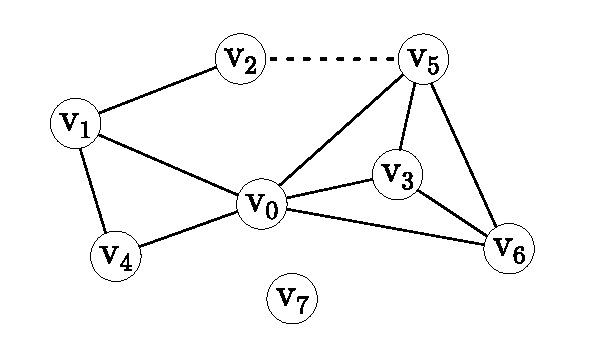
\includegraphics[scale=0.9]{img/graph/chordal.pdf}
	\captionof{figure}[Chordaler Graph]{Der hier abgebildete Graph \( G \) (ohne die gestrichelte Kante) ist chordal.}
	\label{fig:chordalgraph}
\end{minipage}


\section{Perfekte Eliminations-Reihenfolgen}
Um einen Ansatz zur Prüfung der Chordalität eines Graphen zu finden, benötigt man eine äquivalente Aussage, die in diesem Abschnitt hergeleitet werden soll.

\begin{definition}[Vollständiger Graph]
	Ein Graph \( G = \left( V, E \right) \) ist vollständig, wenn jedes Paar \( v, w \in V \) von Knoten durch eine Kante \( \left\lbrace v, w \right\rbrace \in E \) verbunden ist.\footnote{siehe \cite[Kapitel 1.1]{golumbic}}
\end{definition}

Die \textit{Adjazenzmenge} eines Knoten \( x \in V \) bezüglich eines ungerichteten Graphen \( G = \left( V, E \right) \) sei die Menge der Knoten, zu denen \( x \) im Graphen \( G \) eine Verbindung besitzt: \( \textnormal{Adj} \left( x \right) = \left\lbrace y \in V \mid \left\lbrace x, y \right\rbrace \in E \right\rbrace \). Für eine Menge von Knoten \( X \subseteq V \) ist diese \( \textnormal{Adj} \left( X \right) = \bigcup_{x \in X} \textnormal{Adj} \left( x \right) \). Der durch die Teilmenge \( X \subseteq V \) induzierte \textit{Teilgraph} \( G \left[ X \right] \) sei definiert als \( G \left[ X \right] = \left( X, \left\lbrace \left\lbrace v, w \right\rbrace \in E \mid v, w \in X \right\rbrace \right) \).

\begin{definition}[Simplizialer Knoten]
	Ein simplizialer Knoten \( v \) in einem Graphen \( G \) ist ein Knoten, dessen Nachbarn einen vollständigen Teilgraphen \( G \left[\textnormal{Adj} \left( v \right) \right] \) induzieren.\footnote{siehe \cite[Kapitel 4.2]{golumbic}}
\end{definition}

Für den Beweis der nächsten Lemmata benötigen wir folgendes Hilfskonstrukt:

\begin{definition}[Minimaler Knotentrenner]
	Ein Knotentrenner \( S \) der Knoten \( a, b \in V \) ist eine Teilmenge \( S \subseteq V \) mit \( a, b \not\in S \), bei dem sich \( a \) und \( b \) in verschiedenen Zusammenhangskomponenten von \( G \left[ V \setminus S \right] \) befinden.

	\( S \) ist ein minimaler Knotentrenner, falls diese Aussage für kein \( T \subsetneq S \) gilt.\footnote{siehe \cite[Kapitel 4.2]{golumbic}}
\end{definition}

Das folgende Lemma stellt eine bestimmte Eigenschaft von chordalen Graphen dar, die wir in den darauf folgenden Beweisen benötigen:

\begin{lemma}
	Sei \( G = \left( V, E \right) \) ein chordaler Graph. Dann ist der induzierte Teilgraph \( G \left[ S \right] \) zu jedem minimalen Knotentrenner \( S \subseteq V \) vollständig.\footnote{siehe \cite[Satz 4.1 (i) \( \Rightarrow \) (iii)]{golumbic}}
	\label{theorem:seperator}
\end{lemma}

\begin{proof}
	Sei \( S \) ein minimaler Knotentrenner für die Knoten \( a \) und \( b \). \( G \left[ A \right] = \left( A, E_A \right)\) und \( G \left[ B \right] = \left( B, E_B \right)\) seien die Zusammenhangskomponenten von \( G_{V \setminus S} \), die jeweils \( a \) und \( b \) enthalten.

	Da \( S \) minimal ist, hat jeder Knoten \( v \in S \) jeweils einen Nachbarn in \( A \) und \( B \).
	Deshalb existiert zu jedem Knotenpaar \( x, y \in S \) ein minimaler Weg (bezüglich Kantenanzahl) \( \left( x, a_1, a_2, \ldots a_r, y \right) \) mit \( a_i \in A \) und \( \left( y, b_1, b_2, \ldots b_t, x \right) \) mit \( b_i \in B \).

	Der Kreis \( \left( x, a_1, a_2, \ldots, a_r, y, b_1, b_2, \ldots, b_t, x \right) \) besitzt mindestens die Länge \( 4 \) und hat somit, da \( G \) chordal ist, eine Sehne.
	Da die Wege minimal gewählt sind, kann diese jedoch nicht zwei Knoten aus demselben Weg verbinden, womit \( \left\lbrace a_i, a_j \right\rbrace \not\in E\) für \( i, j \in \left\lbrace 1, \ldots r \right\rbrace, \left| i - j \right| > 1 \) und \( \left\lbrace b_i, b_j \right\rbrace \not\in E \) für \( i, j \in \left\lbrace 1, \ldots, t \right\rbrace, \left| i - j \right| > 1 \) gilt. Da alle \( a_i \) und \( b_i \) durch \( S \) getrennt sind, ist außerdem \(\left\lbrace a_i, b_j \right\rbrace \not\in E \) für \( i \in \left\lbrace 1, \ldots, r \right\rbrace \) und \( j \in \left\lbrace 1, \ldots, t \right\rbrace \). Damit müssen die beiden Knoten \( x \) und \( y \) aus dem Knotentrenner verbunden sein.
\end{proof}

Mithilfe von Lemma \ref{theorem:seperator} können wir nun auch folgende Aussage treffen:

\begin{lemma}
	Jeder chordale Graph \( G = \left( V, E \right) \) besitzt einen simplizialen Knoten. Falls \( G \) nicht vollständig ist, dann besitzt dieser zwei nicht-benachbarte simpliziale Knoten.\footnote{siehe \cite[Lemma 4.2]{golumbic}}
	\label{theorem:simplicial}
\end{lemma}

\begin{proof}
	%TODO: Begründen, warum dieser Teilgraph wieder chordal ist

	\begin{itemize}
		\item[Induktionsvoraussetzung:] Für jeden Graphen \( G = \left( V, E \right) \) mit \( \left| V \right| \leq t \) gelte, dass \( G \) entweder vollständig ist oder zwei nicht-benachbarte simpliziale Knoten besitzt.
		\item[\( t = 1 \)] Da ein Graph bestehend aus nur einem Knoten vollständig ist, gilt der Induktionsanfang.
		\item[\( t \Rightarrow t + 1 \)]
		      Sei \( G = \left( V, E \right) \) ein Graph mit \( \left|
		      V \right| = t \) Kanten. Falls \( G \) vollständig ist, ist die Aussage trivial.

		      Habe \( G \) also nun zwei nicht-benachbarte Knoten \( a \) und \( b \) und die Aussage sei für alle Graphen mit weniger Knoten als \( G \) gültig. Wähle als \( S \) einen minimalen Knotentrenner von \( a \) und \( b \); \( G \left[ A \right] \) und \( G \left[ B \right] \) seien wie in Lemma \ref{theorem:seperator} definiert.

		      Wegen der Induktionsvoraussetzung gilt, dass entweder der Teilgraph \( G \left[ A \cup S \right] \) zwei nicht-benachbarte simpliziale Knoten besitzt, von dem einer in \( G \left[ A \right] \) liegen muss (da \( S \) nach Satz \ref{theorem:seperator} vollständig ist) oder \( G \left[A \cup S \right] \) vollständig ist.

		      Da \( \textnormal{Adj} \left( A \right) \subseteq A \cup S \), ist jeder simpliziale Knoten in \( G \left[ A \right] \) ebenfalls simplizial in gesamt \( G \). Mit einer ähnlichen Argumentation lässt sich zeigen, dass auch \( G \left[ B \right] \) einen simplizialen Knoten besitzt.
	\end{itemize}
\end{proof}

Um den Graphen auf Chordalität zu überprüfen, werden wir eine sogenannte perfekte Eliminations-Reihenfolge verwenden, die genau dann existiert, wenn \( G \) chordal ist. Eine \textit{Reihenfolge} ist dabei eine Bijektion \( \sigma: \left\lbrace 1, \ldots, \left| V \right| \right\rbrace \mapsto V \).

\begin{definition}[Perfekte Eliminations Reihenfolge]
	Eine Reihenfolge \( \sigma \) auf \( G = \left( V, E \right) \) ist eine perfekte Eliminations-Reihenfolge, wenn für jedes \( i \in \left\lbrace 1, \ldots, \left| V \right| \right\rbrace \) der Knoten \( \sigma \left( i \right) \) simplizial im Teilgraph \( G \left[ \left\lbrace \sigma \left( i \right), \ldots, \sigma \left( \left| V \right| \right) \right\rbrace \right] \) ist.\footnote{siehe \cite[Kapitel 4.2]{golumbic}}
\end{definition}

\vspace{1em}
\begin{minipage}{\linewidth}
	\centering
	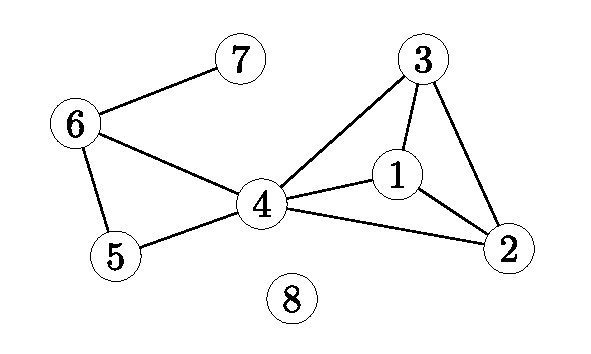
\includegraphics[scale=0.9]{img/graph/peo.pdf}
	\captionof{figure}[Perfekte Eliminations-Reihenfolge]{Die durch die Beschriftung der Knoten dargestellte Reihenfolge \( \sigma \) ist eine perfekte Eliminations-Reihenfolge.}
	\label{fig:peo}
\end{minipage}

Nun ist es uns möglich, die gesuchte Äquivalenz zu beweisen und damit die Hauptaussage des Abschnitts zu zeigen:

\begin{theorem}
	Sei \( G \) ein ungerichteter Graph. \( G \) ist chordal genau dann, wenn für \( G \) eine perfekte Eliminations-Reihenfolge \( \sigma \) existiert.\footnote{siehe \cite[Satz 4.1 (i) \( \Leftrightarrow \) (ii)]{golumbic}}
	\label{theorem:chordalpeo}
\end{theorem}

\begin{proof}
	\begin{itemize}
		\item[\(\Rightarrow\)]
		      Nach Satz \ref{theorem:simplicial} besitzt ein chordaler Graph \( G \) einen simplizialen Knoten \( x \). Da auch \( G \left[ V \setminus \left\lbrace x \right\rbrace \right] \) chordal ist und weniger Knoten als \( G \) besitzt, lässt sich induktiv eine perfekte Eliminations-Reihenfolge erstellen, wenn \( \sigma \) als Reihenfolge der in jedem Schritt entfernten \( x \) gebildet wird.

		\item[\(\Leftarrow\)]
		      Sei \( C \) ein Kreis in \( G \) mit mindestens vier Knoten und \( x \) der kleinste Knoten darin bezüglich \( \sigma^{-1} \left( x \right) \).

		      Durch die Wahl von \( x \) liegt \( C \) vollständig in \( G \left[ \left\lbrace \sigma \left( i \right) \mid i \geq \sigma^{-1} \left( x \right) \right\rbrace \right] \). Da der Knoten \( x \) in diesem Teilgraphen simplizial ist muss zwischen den beiden Nachbarknoten \( v, w \) von \( x \) im Kreis \( C \) eine Sehne existieren.
	\end{itemize}
\end{proof}

\section{Kardinalitätssuche}
\label{section:mcs}
Nachdem wir im vorherigen Kapitel gezeigt haben, dass \( G \) genau dann chordal ist, wenn eine perfekte Eliminations-Reihenfolge \( \sigma \) für \( G \) existiert, werden wir uns in diesem Abschnitt damit beschäftigen, wie sich eine solche perfekte Eliminations-Reihenfolge algorithmisch bestimmen lässt. Dazu werden wir die sogenannte Kardinalitätssuche verwenden, die in der englischen Literatur \textit{Maximum Cardinality Search (kurz MCS)} genannt wird.

Diese wird \glqq{}von hinten\grqq{} gebildet, indem in jedem Schritt \( \sigma \left( i \right) \) mit \( i \in \left\lbrace \left| V \right|, \ldots, 1 \right\rbrace \) jeweils der nicht-nummerierte (also in \( \sigma \) noch nicht zugeordnete) Knoten ist, der am meisten Nachbarn besitzt, die bereits nummeriert worden sind.\footnote{siehe \cite[Kapitel 4.3]{golumbic} und \cite[2.1]{sankardeep}}

Die perfekte Eliminations-Reihenfolge aus Abbildung \ref{fig:peo} hätte dabei durch die Kardinalitätssuche generiert werden können. Diese ist jedoch nicht eindeutig, da in vielen Schritten mehrere Knoten mit größter Zahl an nummerierten Nachbarn verfügbar sind.

\paragraph{Standard-Implementierung} Eine einfache Implementierung basiert darauf, die Knoten nach der Anzahl der benachbarten, nummerierten Knoten in Mengen sortiert zu halten:

Als Datenstruktur wird ein Array \( \texttt{S} \) von \( n = \left| V \right| \) Mengen verwendet, in dem alle nicht-num\-mer\-ier\-ten Knoten gespeichert sind. Dabei sind jeweils in \( \texttt{S} \left[ i \right] \) die Knoten mit \( i \) nummerierten Nachbarn zu finden (\( i \in \left\lbrace 0, \ldots, n - 1 \right\rbrace \)). Um in konstanter Zeit auf Knoten in \( \texttt{S} \) zugreifen zu können und den Index der Menge zu finden, benötigen wir zusätzlich dazu noch zwei Listen von Zahlen: Während in \( \texttt{M} \) für jeden Knoten \( v \in V \) die Position in \( \texttt{S} \) gespeichert wird, sind es in \( \texttt{N} \) jeweils die Anzahl der nummerierten Nachbarn und somit auch der Index der Menge in \( \texttt{S} \).\footnote{siehe \cite[Abschnitt 2, Algorithmus Maximum Cardinality Search]{tarjanyannakakis}, nur, dass in \( \texttt{M} \) nun die genaue Position in \( \texttt{S} \) gespeichert wird, vergleichbar mit \cite[Abschnitt 2]{sankardeep}}

Da in \( \texttt{M} \) und \( \texttt{N} \) für alle \( n \) Knoten die in \( \mathcal{O} \left( \textnormal{lg} \left( n \right) \right)\) bits darstellbare Position in \( \texttt{S} \) gespeichert ist, genügen hier jeweils \( \mathcal{O} \left( n \cdot \textnormal{lg} \left( n \right) \right) \) Speicher. \( \texttt{S} \) lässt sich dabei durch einen Array von \( n \) doppelt-verketteten Listen darstellen, deren einzelne Einträge sich mit jeweils \( \mathcal{O} \left( \textnormal{lg} \left( n \right) \right) \) bits speichern lassen, womit insgesamt hier ebenfalls \( \mathcal{O} \left( n \cdot \textnormal{lg} \left( n \right) \right) \) bits ausreichen.\footnote{siehe \cite{sankardeep}}

Zu Beginn der Ausführung werden alle Knoten von \( G \) in \( \texttt{S} \left[ 0 \right] \) eingetragen und in \( \texttt{M} \) und \( \texttt{N} \) entsprechend gegenreferenziert. In jedem Schritt \( i \in \left\lbrace n, \ldots, 1 \right\rbrace \) wird dann das Element \( \sigma \left( i \right) \) bestimmt: Dieses ist ein beliebiger Knoten \( v \in \texttt{S} \left[ j \right]\), wobei \( j \) der größte Index einer Menge in \( \texttt{S} \) ist, für den \( \texttt{S} \left[ j \right] \neq \emptyset \). Anschließend wird jeder nicht-nummerierte Nachbarknoten \( w \) von \( v \) aus der Menge \( \texttt{S} \left[ \texttt{N} \left[ w \right] \right] \) entfernt und in \( \texttt{S} \left[ \texttt{N} \left[ w \right] + 1 \right] \) eingefügt und dann auch jeweils die Gegenreferenzen in \( \texttt{N} \) und \( \texttt{M} \) aktualisiert.

\begin{algorithm}
	\SetAlgoVlined
	\KwData{Graph \( G = \left( V, E \right) \)}
	\For{\( i \in \left\lbrace 0, \ldots, n-1 \right\rbrace  \)}{
		\( \texttt{S}\left[ i \right] \longleftarrow \emptyset \)
	}
	\For{\( v \in V \)}{
		füge \( v \) in \( \texttt{S} \left[ 0 \right]\) ein\;
		\( \texttt{M} \left[ v \right] \longleftarrow \) Position von \( v \) in \( \texttt{S}\left[ 0 \right] \)\;
		\( \texttt{N} \left[ v \right] \longleftarrow 0 \)\;
	}
	\( j \longleftarrow 0 \)\;
	\For{\( i \in \left\lbrace n, \ldots, 1 \right\rbrace \)}{
		\( v \longleftarrow\) entferne einen Knoten aus \(  \texttt{S}\left[ j \right] \)\;
		\( \sigma\left[ i \right] \longleftarrow v\)\;
		\( j \longleftarrow j + 1\)\;
                \( \textnormal{\texttt{N}}\left[ v \right] \longleftarrow -1\)\;
		\For{\( w \in \textnormal{Adj}\left( v \right)\) mit \( \textnormal{\texttt{N}}\left[ w \right] \geq 0 \) }{
			\( k \longleftarrow N \left[ w \right] \)\;
			lösche \( w \) aus \( \texttt{S} \) an Position \(\texttt{M}\left[ w \right]\) aus der Menge \( \texttt{S}\left[ k \right] \)\;
			füge \( w \) in \( \texttt{S}\left[ k + 1 \right] \) ein\;
			\( \texttt{N} \left[ w \right] \longleftarrow k + 1 \)\;
			\( \texttt{M}\left[ w \right] \longleftarrow \) neue Postion von \( v \) in \( \texttt{S}\left[ k \right] \)\;
		}
		\While{\(j \geq 0 \land \textnormal{\texttt{S}}\left[ j \right] = \emptyset \)}{
			\( j \longleftarrow j - 1 \)\;
		}
	}
	\KwResult{Reihenfolge \( \sigma: \left\lbrace 1, \ldots, n \right\rbrace \mapsto  V \) der Knoten in \( V \)}
	\caption{Kardinalitätssuche nach \cite[2.1]{sankardeep}}
	\label{algorithm:defaultmcs}
\end{algorithm}

Eine Implementierung in Pseudo-Code ist in Algorithmus \ref{algorithm:defaultmcs} zu finden. Dabei ist vor allem die Verwaltung des Index der größten Menge \( j \) interessant. Am Anfang wird dieser auf \( 0 \) gesetzt, da sich alle Elemente in \( \texttt{S} \left[ 0 \right] \) befinden. Da der Index der Menge in \( \texttt{S} \) eines Knotens in jedem Schritt um maximal \( 1 \) erhöht werden kann, wird  \( j \) um \( 1 \) inkrementiert, um sicherzustellen, dass \( j \geq \textsf{max} \left\lbrace j \in \left\lbrace 1, \ldots, n \right\rbrace | \texttt{S} \neq \emptyset \right\rbrace \). Mithilfe der \textbf{while}-Schleife wird diese Ungleichung dann wieder zur Gleichung.

Bei der Ausführung werden dann zuerst alle Knoten in \( \texttt{S} \left[ 0 \right] \) eingefügt und entsprechend in \( \texttt{M} \) gegenreferenziert, was \( \mathcal{O} \left( n \right) \) Zeit benötigt. Anschließend werden für jeden der \( n \) Knoten jeweils die Adjazenzliste durchlaufen; dies kann in \(\mathcal{O}\left( \sum_{v \in V} \left(1 + \left| \textnormal{Adj} \left( v \right) \right| \right) \right) = \mathcal{O} \left( n + m \right) \) erreicht werden. Da \( j \) in jedem der \( n \) Durchläufe um jeweils \( 1 \) inkrementiert wird, und nie \( j < -1 \) gelten kann, wir der Rumpf der \textbf{while}-Schleife höchstens \( n + 1\) mal durchlaufen, sodass alle Operationen auf \( j \) höchstens \( \mathcal{O} \left( n \right) \) Zeit benötigen. Damit ist die gesamte Laufzeit des Algorithmus' \( \mathcal{O} \left( n + m \right) \).

Um nun zu beweisen, dass die Kardinalitätssuche wirklich -- falls dies möglich ist, also \( G \) chordal ist -- eine perfekte Eliminations-Reihenfolge bestimmt, beweisen wir zunächst, dass jede von der Kardinalitätssuche generierte Reihenfolge folgende Eigenschaft besitzt:

\begin{definition}[Reihenfolgeneigenschaft \( P \)]
	Sei \( \sigma \) eine Reihenfolge der Knoten des Graphen \( G = \left( V, E \right) \).

	\( \sigma\) besitzt die Eigenschaft \( P \), falls für alle Knoten \( a, b, c \in V \) mit \( \sigma^{-1} \left( a \right) < \sigma^{-1} \left( b \right) < \sigma^{-1} \left( c \right)\) und \( c \in \textnormal{Adj} \left( a \right) \setminus \textnormal{Adj} \left( b \right) \) ein weiterer Knoten \( x \in \textnormal{Adj} \left( b \right) \setminus \textnormal{Adj} \left( a \right) \) mit \( \sigma^{-1} \left( b \right) < \sigma^{-1} \left( x \right) \) existiert.\footnote{siehe \cite[Lemma 4]{tarjanyannakakis}}
\end{definition}

\begin{theorem}
	Jede von der Kardinalitätssuche generierte Reihenfolge \( \sigma \) besitzt die Eigenschaft \( P \).\footnote{siehe \cite[Satz 2]{tarjanyannakakis}}
	\label{theorem:mcserfuelltp}
\end{theorem}

\begin{proof}
	Sei \( \sigma \) eine Reihenfolge der Knoten des Graphen \( G = \left( V, E \right) \), die durch die Kardinalitätssuche berechnet wurde.

	Seien \( a, b, c \in V \) mit den Eigenschaften \( \sigma^{-1}\left( a \right) < \sigma^{-1}\left( b \right) < \sigma^{-1}\left( c \right) \),  \( \left\lbrace a, c \right\rbrace \in E \) und \( \left\lbrace c, b \right\rbrace \not\in E \).

	In dem Moment, in dem bei der Ausführung der Kardinalitätssuche \( b \) nummeriert wird, muss \( b \) zu mindestens genauso vielen bereits nummerierten Knoten benachbart sein wie \( a \).  Folglich, da \( a \) (aber nicht \( b \)) mit \( c \) verbunden ist, ist \( b \) benachbart zu einem anderen zuvor nummerierten Knoten \( x\), der nicht mit \( a \) verbunden ist. Da dies für beliebige \( a \), \( b \) und \( c \) gilt, besitzt die gesamte Sortierung \( \sigma\) die Eigenschaft \( P \).
\end{proof}

Um bewiesen zu haben, dass mit der Kardinalitätssuche wirklich eine perfekte Eliminations-Rei\-hen\-fol\-ge berechnet wird, fehlt somit noch folgende Aussage:

\begin{theorem}
	Sei \( G \) ein chordaler Graph.\\
	Falls die Reihenfolge \( \sigma \) von den Knoten von \( G \) die Eigenschaft \( P \) erfüllt, so ist \( \sigma \) eine perfekte Eliminations-Reihenfolge.\footnote{siehe \cite[Lemma 4]{tarjanyannakakis} mit für perfekte Eliminationsreihenfolgen abgewandeltem Beweisende}
	\label{theorem:auspfolgtchordal}
\end{theorem}

\begin{proof}
	Sei \( \sigma \) eine Reihenfolge der Knoten des chordalen Graphen \( G = \left( V, E \right) \), die die Eigenschaft \( P \) aufweist.

	Ein Weg \( \pi = \left( v_0, \ldots, v_k \right) \) in \( G \) mit \( k \geq 2 \) besitzt die Eigenschaft \( Q \) genau dann, wenn folgende Aussagen erfüllt sind:

	\begin{itemize}
		\item \( \pi \) besitzt keine Zwischenverbindungen (für beliebige \( i, j \in \left\lbrace 1, \ldots k \right\rbrace, \left| i - j \right| \neq 1 \) gelte \( \left\lbrace v_i, v_j\right\rbrace \not\in E \)).
		\item Für ein \( i \in \left\lbrace 1, 2, \ldots, k - 1 \right\rbrace \) sei \( \sigma^{-1} \left( v_0 \right) > \sigma^{-1} \left( v_k \right) > \sigma^{-1} \left( v_1 \right)  >  \sigma^{-1} \left( v_2 \right) > \ldots > \sigma^{-1} \left( v_i \right) \) und \( \sigma^{-1} \left( v_i \right) < \sigma^{-1} \left( v_{i + 1} \right) < \ldots < \sigma^{-1} \left( v_k \right) \).
	\end{itemize}

	Unser Ziel ist nun zu zeigen, dass ein solcher Weg mit Eigenschaft \( Q \) nicht existieren kann: Dazu nehmen wir an, das \( \pi \) so gewählt ist, dass es keinen Pfad mit größerem \( \sigma^{-1} \left( v_k \right) \) gibt, der \( Q \) erfüllt.

	Da \( \pi \) keine Zwischenverbindung besitzt, sind zwar \( v_0 \) und \( v_1 \) benachbart, aber \( v_0 \) und \( v_k \) nicht. Da durch \( Q \) die Ungleichung \( \sigma^{-1} \left( v_1 \right) < \sigma^{-1} \left( v_k \right) < \sigma^{-1} \left( v_0 \right) \) gilt, existiert nach \( P \) ein Knoten \( x \) mit \( \sigma^{-1} \left( v_k \right) < \sigma^{-1} \left( x \right) \), der zu \( v_k \), aber nicht zu \( v_1 \), benachbart ist.

	Sei \( j > 0 \) minimal mit \( v_j \in \textnormal{Adj} \left( x \right) \). \( x \) ist nicht zu \( v_0 \) benachbart, da sonst \( \left( x, v_0, v_1, \ldots, v_j, x \right) \) ein Kreis ohne Sehne wäre, was der Chordalität von \( G \) widersprechen würde. Falls nun \( \sigma^{-1} \left( v_0 \right) > \sigma^{-1} \left( x \right) \) gelten würde, besäße \( \left( v_0, v_1, \ldots, v_j, x\right) \) die Eigenschaft \( Q \); im anderen Fall \( \sigma^{-1} \left( v_0 \right) < \sigma^{-1} \left( x \right) \) wäre es \( \left( x, v_{j}, v_{j-1}, \ldots, v_0 \right) \).

	Dies steht im Widerspruch dazu, dass \( \sigma^{-1} \left( v_k \right) \) maximal gewählt ist, womit kein Pfad die Eigenschaft \( Q \) besitzen kann.

	Betrachte nun mit \( i \in \left\lbrace 1, \dots, \left| V \right| \right\rbrace \) beliebig den Knoten \( \sigma \left( i \right) \). Um zu beweisen, dass \( \sigma \) eine perfekte Eliminations-Reihenfolge ist, muss hier somit gezeigt werden, dass \( \sigma \left( i \right) \) in dem Teilgraphen \( G \left[ \left\lbrace \sigma \left( i \right), \ldots, \sigma \left( \left| V \right| \right) \right\rbrace \right] \) simplizial ist:

	Seien also \( v, w \in \textnormal{Adj} \left( \sigma \left( i \right) \right), v \neq w \) mit \( i < \sigma^{-1} \left( v \right) \) und \( i < \sigma^{-1} \left( w \right) \) . \( v \) und \( w \) sind somit benachbart, da sonst entweder die Wege \( \left( v, \sigma \left( i \right), w \right) \) oder \( \left( w, \sigma \left( i \right), v \right) \) die Eigenschaft \( Q \) erfüllen würden.
\end{proof}

\begin{corollary}
	Ein Graph \( G = \left( V, E \right) \) ist genau dann chordal, wenn die von der Kardinalitätssuche auf \( G \) generierte Ordnung \( \sigma \) eine perfekte Eliminations-Reihenfolge ist.
\end{corollary}

\begin{proof}
	\begin{itemize}
		\item[\( \Rightarrow \)]
		      Für eine von der Kardinalitätssuche auf einem chordalen Graphen \( G \) generierte Reihenfolge \( \sigma \) wurde in Satz \ref{theorem:mcserfuelltp} gezeigt, dass diese \( P \) erfüllt. Daraus folgt nach Satz \ref{theorem:auspfolgtchordal}, dass es sich bei \( \sigma \) um eine perfekte Eliminations-Reihenfolge handelt.
		\item[\( \Leftarrow \)]
		      Wenn ein von der Kardinalitätssuche auf \( G \) generiertes \( \sigma \) eine perfekte Eliminationsreihenfolge ist, folgt mithilfe der Äquivalenz aus Satz \ref{theorem:chordalpeo}, dass \( G \) chordal ist.
	\end{itemize}
\end{proof}

Um einen Graphen \( G \) auf Chordalität zu überprüfen, können wir somit zuerst mithilfe der Kardinalitätssuche die Reihenfolge \( \sigma \) berechnen, und müssen anschließend noch überprüfen, ob es sich bei \( \sigma \) um eine perfekte Eliminations-Reihenfolge handelt. Genauer beschrieben wird dieser letzte Schritt beispielsweise in \cite[Algorithmus 4.2]{golumbic}, der mit \( \mathcal{O} \left( \left| V \right| + \left| E \right| \right) \) Zeit auskommt.

\section{Zeit- / Platz-Tradeoffs für die Kardinalitätssuche}
Der in Abschnitt \ref{section:mcs} vorgestellte Algorithmus besitzt zwar eine lineare Laufzeit, verwendet aber mit \(\mathcal{O}\left( n \cdot \textnormal{lg} \left( n \right) \right) \) bits relativ viel Speicher. Dies kann vor allem dann störend werden, wenn Zeit keine Priorität ist und große Datenmengen mit einem kleinen beschreibbaren Arbeitsspeicher verarbeitet werden sollen (beispielsweise auf eingebetteten Systemen). Deshalb werden in \cite{sankardeep} platzeffizientere Varianten der Kardinalitätssuche vorgestellt, die dafür eine längere Laufzeit besitzen:

Im Folgenden wird nun das Rechnermodell formal definiert, das auch schon implizit in Abschnitt \ref{section:mcs} verwendet wurde:

\paragraph{Rechnermodell und Datenformat} Zur Ausführung und Analyse der Algorithmen in dieser Arbeit wird das \textit{Random Access Machine}-Modell verwendet, wobei für die Ausführung ein beliebig les- und beschreibbarer Speicher mit einer bestimmten Grö\-ßen\-ord\-nung zur Verfügung steht. Die für Adressierung eines Knotens benötigte Wortgröße liegt dabei in \( \mathcal{O} \left( \textnormal{lg} \left( n \right)\right) \) Bits.

Der Eingabegraph \( G \) mit seinen \( n \) Knoten und \( m \) Kanten ist in einem nur lesbaren separaten Speicher zu finden. Die Kanten sind als Adjazenzlisten \(\textnormal{Adj} \left( x \right) \)  verfügbar, womit ein beliebiger Nachbar eines Knotens \( x \in V \) in \( \mathcal{O} \left( 1 \right) \) Zeit ausgewählt werden kann.

Für die Ausgabe wird ein separater Speicher verwendet, aus dem bereits geschriebene Ausgaben weder gelesen noch verändert werden können.\footnote{Rechnermodell von \cite{sankardeep}, genauer spezifiziert in \cite{asano}} In dieser Arbeit wird der Ausgabespeicher beginnend mit dem letzten Element von \( \sigma \) beschrieben. Bei einem nur sequentiell beschreibbaren Ausgabespeicher würden damit bei der Verwendung dieser Algorithmen eine umgekehrte perfekte Eliminations-Reihenfolge berechnet werden können und damit zusätzliche Zeit und Kosten für das Umkehren der Reihenfolge anfallen.

\begin{algorithm}
	\SetAlgoVlined
	\KwData{Graph \( G = \left( V, E \right) \)}
	\For{\( v \in V  \)}{
		\( \texttt{B}\left[ v \right] \longleftarrow \textnormal{\texttt{false}} \)\;
	}
	\For{\( i \in \left\lbrace n, \ldots, 1 \right\rbrace \)}{
		\(u \longleftarrow \textnormal{wähle beliebigen Knoten } x \in V \)\;
		\(c \longleftarrow 0 \)\;
		\For{\( v \in V \) mit \(\textnormal{\texttt{B}} \left[ v \right] = \textnormal{\texttt{false}}\)}{
			\( k \longleftarrow 0 \)\;
			\For{\( w \in  \textnormal{Adj} \left( v \right)\) mit \(\textnormal{\texttt{B}}\left[ w \right] = \textnormal{\texttt{true}}\)}{
				\( k \longleftarrow k + 1 \)\;
			}
			\If{\( k \geq c \)}{
				\(u \longleftarrow v\)\;
				\(c \longleftarrow k\)\;
			}
		}
		\(\textnormal{\texttt{B}} \left[ u \right] = \textnormal{\texttt{true}}\)\;
		\(\sigma \left[ i \right] \longleftarrow u\)\;
	}
	\KwResult{Reihenfolge \( \sigma: V \mapsto \left\lbrace 1, \ldots, n \right\rbrace \) der Knoten in \( V \)}
	\caption{Kardinalitätssuche mit \( n + \mathcal{O} \left( \textnormal{lg} \left( n \right) \right) \text{bits} \) Speicher nach \cite[3.1]{sankardeep}}
	\label{algorithm:mcsb}
\end{algorithm}

\paragraph{\( n + \mathcal{O} \left( \textnormal{lg} \left( n \right) \right) \text{bits} \)}
Bei dieser sehr speicher-fokussierten Realisierung der Kar\-di\-na\-li\-täts\-suche verwenden wir nur ein Bit-Array \( \texttt{B} : V \mapsto \left\lbrace \texttt{true}, \texttt{false} \right\rbrace \) und Zählvariablen zum Iterieren der Knoten. Somit werden \( n \text{ bits} \) für die Knoten und jeweils \( \textnormal{lg} \left( n \right) \) bits für die Zählvariablen benötigt, also insgesamt \( n + \mathcal{O} \left( \textnormal{lg} \left( n \right) \right) \text{bits}\).

Zu Beginn wird der gesamte Array \( \texttt{B} \) mit \( \texttt{false} \) (für nicht markiert) initialisiert.

Anschließend wird \( \sigma \) mit dem letzten Element beginnend schrittweise berechnet:
In jedem Durchlauf \( i \in \left\lbrace n, \ldots, 1 \right\rbrace \) wird für jedes \( v \in V \) geprüft, ob es noch nicht nummeriert wurde, also ob \( \texttt{B}\left[ v \right] = \texttt{false} \). Falls ja, wird die Adjazenzliste \( \textnormal{Adj}\left( v \right) \) durchlaufen und die Anzahl der Elemente darin gezählt, die bereits nummeriert sind (also
\( \texttt{B} = \texttt{true} \)). Dabei wird der Knoten \( u \) mit der in dem jeweiligen Schritt größten Anzahl an nummerierten Nachbarn bestimmt und anschließend so in die Position von \( \sigma \left( i \right) \) des Ausgabespeichers geschrieben -- womit er am Anfang der bereits berechneten Einträge steht. In Algorithmus \ref{algorithm:mcsb} ist dieses Vorgehen als Pseudo-Code zusammengefasst.

Da für jeden der \( n \) Knoten in jedem Schritt einmal alle Adjazenzlisten durchlaufen werden (was \(O\left( m\right)\) Zeit benötigt), hat diese Variante eine Laufzeit von \( \mathcal{O} \left( n \cdot m \right) \).\footnote{siehe \cite[Abschnitt 3.1]{sankardeep}}

\paragraph{\( \mathcal{O} \left( n \right) \text{ bits} \)} Die folgende Version der Kardinalitätssuche verwendet deutlich mehr Speicher (\( \mathcal{O} \left( n \right) \) statt \( n \) bits):

Neben dem Bit-Vektor \( \texttt{B} \)  werden hier weitere Datenstrukturen zum Speichern der Knoten verwendet: In der doppelt verketteten Liste \( \texttt{L} \) besteht jedes Element aus einer Zahl \( \texttt{labeledNeighbors} \) für die Anzahl der nummerierten Nachbarn und einer weiteren verketteten Liste von Knoten, deren Einträge jeweils \( \texttt{labeledNeighbors} \) nummerierte Nachbarn besitzen. Um Platz zu sparen, werden immer nur \( s \in \Theta \left( \frac{n}{\textnormal{lg}\left( n \right)}\right) \) Elemente in \( \texttt{S} \) und \( \texttt{T} \) gehalten. Die äußere Liste ist nach \( \texttt{labeledNeighbors} \) sortiert; auf das jeweils erste und letzte Element kann in \( \mathcal{O} \left( 1 \right) \) zugegriffen werden. Um auf einen Knoten innerhalb der geschachtelten Liste innerhalb von \( \mathcal{O} \left( \textnormal{lg} \left( n  \right) \right) \) zugreifen zu können, wird außerdem ein Suchbaum \( \texttt{T} \)  angelegt, in dem alle Knoten zu finden sein sollen, die auch in \( \texttt{L} \) sind. Bei den Knoten in \( \texttt{L} \) und \( \texttt{T} \) sind Zeiger auf diese in der jeweils anderen Struktur eingetragen.

Da jeder Knoten mit \( \mathcal{O} (\textnormal{lg}\left( n \right)) \) bits in den Datenstrukturen \( \texttt{L} \) und \( \texttt{T} \) gespeichert werden kann und maximal \( \Theta \left(\frac{n}{\textnormal{lg}\left( n \right)} \right) \) Knoten auf einmal geladen sind, wird für beide Strukturen \( \mathcal{O} \left( n \right) \) Bits Speicher benötigt. \( \texttt{B} \) hat mit \( n \) Bits einen geringeren Speicherbedarf - womit hier insgesamt \( \mathcal{O} \left( n \right) \) bits ausreichen.

Bei der Ausführung des Algorithmus' werden zuerst \( s \) Knoten in \( \texttt{L} \) und \( \texttt{T} \) geladen, bei \( \texttt{L} \) kommen dabei alle Knoten in die Liste mit \( \texttt{labeledNeighbors} = 0 \). \( \texttt{B} \) wird wieder komplett mit \( \texttt{false} \) initialisiert.

Im \( i \)-ten Schritt wird zuerst ein Knoten \( v \) aus \( \texttt{L} \) aus der Unterliste mit dem größten \( \texttt{labeledNeighbors} \) genommen. Dieser wird dann in \( \sigma \) in die Position \( \sigma \left( n - i + 1\right) \) angefügt, in \( \texttt{B} \) als nummeriert markiert und anschließend aus \( \texttt{L} \) und \( \texttt{T} \) entfernt. Falls dadurch die entsprechende Liste, aus der der Knoten entfernt wurde, leer wird, wird das entsprechende Element aus \( \texttt{L} \) gelöscht.

Für jeden Nachbarn von \( w \in \textnormal{Adj} \left( v \right) \) wird anschließend zuerst geprüft, ob sich dieser bereits in \( \texttt{T} \) (und somit auch \( \texttt{L} \)) befindet.
Falls ja, wird dieser in das (eventuell neu erstellte) Listenelement von \( \texttt{L} \) mit einem um eins höheren \texttt{labeled\-Neighbors} eingefügt und aus seiner alten Unterliste entfernt. Zusätzlich wird die Referenz in \( \texttt{T} \) aktualisiert.
Falls dieser noch nicht in \( \texttt{T} \) vorhanden ist, wird zuerst mithilfe von \( \texttt{B} \) die Anzahl der nummerierten Nachbarn bestimmt und in einer Variable \( k \) gespeichert. Falls diese Zahl größer ist als das kleinste \( \texttt{labeledNeighbors} \) in \(\texttt{L}\), wird der Knoten in die entsprechende (eventuell neu erstellte) Unterliste mit \texttt{labeled\-Neighbors} \( = k\) von \( \texttt{L} \) eingefügt, und - falls sonst die Maximalanzahl von \( s \) Knoten überschritten werden würden - der erste Knoten aus der Liste mit dem kleinsten \( \texttt{labeledNeighbors} \) in \( \texttt{L} \) (und \( \texttt{T}\)) entfernt.

Wenn während der Ausführung die in \( \texttt{L} \) und \( \texttt{T} \) zwischengespeicherten Knoten ausgehen, werden wieder \( s \) neue, nicht-nummerierte Knoten nachgeladen (soweit vorhanden). Das Einfügen der ersten \( s \) Knoten erfolgt für jeden der Knoten \( v \), indem die  Nachbarn \( w \in \textnormal{Adj} \left( v \right) \) mit \( \texttt{B}\left[w\right] = \texttt{true} \) gezählt werden (diese Anzahl sei \( k \)) und anschließend \( v \) in die (eventuell neu erstellte Liste) mit \( \texttt{labeledNeighbors} = k \) eingefügt wird. Bei den restlichen Knoten wird genauso die Anzahl \( k \) der benachbarten, nummerierten Knoten berechnet, und falls diese größer ist als das kleinste vorhandene \( \texttt{labeledNeighbors} \) bei einem Element von \( \texttt{L} \), wird ein Knoten aus der Liste mit dem kleinsten \( \texttt{labeledNeighbors} \) durch diesen wie bereits beschrieben ersetzt.

Bestimmen wir im Folgenden die Laufzeit dieser Variante der Kardinalitätssuche:

Bei einem Nachfüllen von \( \texttt{L} \) wird das Hinzufügen von einem Knoten durch die Zeit zum Durchlaufen der Nachbarn dominiert - und lässt sich somit mit \( \mathcal{O} \left( m \right) \) abschätzen. Da das Nachfüllen der Liste höchstens \( \textnormal{lg} \left( n \right) \) mal passiert, hat dies insgesamt eine Laufzeit von \( \mathcal{O} \left( m \cdot \textnormal{lg} \left( n \right) \right) \).

Das darauf folgende Einfügen der \( s \in \Theta \left( \frac{\textnormal{lg} \left( n \right) }{n} \right) \) Knoten in den balancierten Baum \( \texttt{T} \) kostet jeweils \( \mathcal{O} \left( \textnormal{lg} \left( n \right) \right) \) Zeit, somit werden dafür insgesamt \( \mathcal{O} \left( n \right) \) Rechenschritte benötigt.

Da bei jedem Verschieben von Knoten zwischen Listen ein solcher zuerst mit \( \mathcal{O} \left( \textnormal{lg} \left( n \right) \right)\) Aufwand in \( \texttt{T} \) gesucht werden muss, ist die Laufzeit für das Verschieben von Knoten \( \mathcal{O} \left( \textnormal{lg} \left( n \right) \right)\). Ein Knoten muss maximal \( \left| \textnormal{Adj}\left( v \right) \right| \) mal verschoben werden (jedes Mal, wenn ein Nachbar nummeriert wird) - dies passiert maximal \( \mathcal{O} \left( \sum_{w \in V} \left| \textnormal{Adj}\left( w \right) \right| \right)  = \mathcal{O} \left( m \right)\) mal. Damit betragen die Laufzeitkosten dafür insgesamt \( \mathcal{O} \left( m \cdot \textnormal{lg} \left( n \right) \right) \).

Beim Berechnen der Anzahl der nummerierten Nachbarn eines Knoten \( v \) muss jeweils die Adjazenzliste durchlaufen werden (\(\mathcal{O} \left( \left| \textnormal{Adj}\left( v \right) \right| \right) \) Zeit) - und da dies bei der Nummerierung jedes Nachbarn passieren kann, ergibt sich dafür insgesamt eine Laufzeit von \( \mathcal{O} \left( \sum_{w \in V} \left| \textnormal{Adj}\left( w\right) \right|^2 \right) \) Rechenschritten.

Die Autoren von \cite{sankardeep} haben dies mit \( \mathcal{O} \left( \sum_{w \in V} \left| \textnormal{Adj}\left( w\right) \right|^2 \right)  = \mathcal{O} \left( \frac{m^2}{n}\right)\) abgeschätzt. Dass diese Abschätzung nicht funktioniert, kann man an folgendem Beispiel erkennen:

Sei \( G = \left( V, E \right) \) ein sternförmiger Graph, also mit \( V = \left\lbrace v_1, \ldots, v_n \right\rbrace \) und \[ E = \left\lbrace \left\lbrace v_1, v_2 \right\rbrace, \ldots, \left\lbrace v_1, v_n \right\rbrace \right\rbrace. \] Dann ergibt sich für die linke Seite \( \sum\limits_{v \in V} {\left| \textnormal{Adj}\left( v\right) \right}^2 = 1 \cdot \left( n -1 \right)^2 + \left( n - 1 \right) \cdot 1^2 \in \mathcal{O} \left( n^2 \right) \) und für die rechte Seite \( \frac{\left( n - 1 \right)^2}{n} \in \mathcal{O} \left( n \right) \), womit eine Gleichheit der Mengen nicht gegeben sein kann.

Eine gültige Abschätzung wäre \[ \mathcal{O} \left( \sum_{w \in V} \left| \textnormal{Adj}\left( w\right) \right|^2 \right) \subseteq \mathcal{O} \left( \sum_{v \in V} \sum_{w \in V} \left| \textnormal{Adj}\left( v\right) \right| \cdot \left| \textnormal{Adj}\left( w\right) \right| \right) = \mathcal{O} \left( m^2 \right), \] die im Falle des beschriebenen sternförmigen Graphen eine Gleichheit wäre.

Die daraus resultierende Gesamtlaufzeit von \( \mathcal{O} \left( m^2 + m \cdot \textnormal{lg} \left( n \right)\right) \) (statt \( \mathcal{O} \left( \frac{m^2}{n} + m \cdot \textnormal{lg} \left( n \right)\right) \))\footnote{siehe \cite[Abschnitt 3.2]{sankardeep}} besitzt jedoch schon bei Graphen mit \( m \in \mathcal{O} \left( n \right) \) mit dieser Abschätzung eine schlechtere Laufzeit als die platzsparendere erste Version.

Zusammengefasst ergeben sich durch die beschriebenen Algorithmen folgende Zeit- / Speicherplatz-Tradeoffs:

\begin{theorem}
	Es ist möglich, für einen Graphen \( G = \left( V, E \right) \) mit \( n = \left| V \right| \) Knoten und  \( m = \left| E \right| \) Kanten eine perfekte Eliminations-Reihenfolge \( \sigma \) zu erhalten in\footnote{siehe \cite[Satz 1]{sankardeep} (Option c wurde hier ersetzt durch den Stan\-dard-Al\-go\-rith\-mus)}
	\begin{enumerate}[a)]
		\item \( \mathcal{O} \left( n \cdot m \right) \) Zeit mit \( n + \mathcal{O} \left( \textnormal{lg} \left( n\right) \right) \) bits
		\item \( \mathcal{O} \left( m ^ 2 + m \cdot \textnormal{lg} \left( n\right) \right) \) Zeit mit \( \mathcal{O} \left( n \right) \) bits
		\item \( \mathcal{O} \left( n + m \right) \) Zeit mit \( \mathcal{O} \left( n \cdot \textnormal{lg} \left( n \right) \right) \) bits
	\end{enumerate}
\end{theorem}

\section{Anwendung beim Gauß-Algorithmus}
Eine praktische Anwendung von chordalen Graphen und perfekten Eliminations-Rei\-hen\-fol\-gen ist eine Möglichkeit zum Beschleunigen des dem Leser bereits bekannten Gauß-Algorithmus\footnote{beispielsweise erklärt in \cite[Abschnitt 3.3]{stykel}} auf dünnbesetzten Matrizen.

Eine \textit{dünnbesetzte} Matrix ist eine Matrix, die deutlich mehr \( 0 \)-Einträge als Einträge mit anderen Zahlen besitzt. Um sich Rechenoperationen bei der Ausführung des Gauß-Algorithmus zu sparen, ist es dabei von Interesse, diese \( 0 \)-Einträge zu erhalten, da diese Einträge bei den Zeilenadditionen  - falls man nur die Nicht-\( 0 \)-Einträge zusammen mit ihren Positionen speichert - ausgelassen werden können, und damit zusätzlich weniger Speicherplatz für die Matrix benötigt wird.

Für das folgende Beispiel werden wir diese symmetrische \( 8 \times 8 \)-Matrix betrachten, deren Diagonale vollständig besetzt ist\footnote{\( A \) muss symmetrisch sein, damit der später daraus generierte Graph ungerichtet ist. Die Diagonalen müssen \( \neq 0 \), damit der Gauß-Algorithmus ohne Zeilenvertauschungen auskommt.}:

\[
	A =
	\begin{bmatrix}
		9 & 2 & 0 & 2 & 1 & 1 & 2 & 0 \\
		2 & 8 & 2 & 0 & 1 & 0 & 0 & 0 \\
		0 & 2 & 7 & 0 & 0 & 0 & 0 & 0 \\
		2 & 0 & 0 & 8 & 0 & 1 & 3 & 0 \\
		1 & 1 & 0 & 0 & 9 & 0 & 0 & 0 \\
		1 & 0 & 0 & 1 & 0 & 7 & 2 & 0 \\
		2 & 0 & 0 & 3 & 0 & 2 & 9 & 0 \\
		0 & 0 & 0 & 0 & 0 & 0 & 0 & 8
	\end{bmatrix}
\]

Die genauen Einträge von \( A \) sind hier so gewählt, dass bei der Ausführung des Gauß-Algorithmus keine \( 0 \) in einer Spalte entsteht, die nicht gerade eliminiert wird. Dies stellt sicher, dass immer ein Pivotelement ohne Vertauschung gefunden werden kann.

Wenn wir darauf den Gauß-Algorithmus ausführen (Abbildung \ref{fig:gauss01}), werden im Laufe der Berechnung zusätzlich zu den bereits in der Originalmatrix vorhandenen Nicht-\( 0 \)-Einträgen \begin{tikzpicture}\fill[fill=black] circle(0.7ex);\end{tikzpicture} einige weitere entstehen \begin{tikzpicture}\fill[fill=red] circle(0.7ex);\end{tikzpicture}.

\begin{figure}
	\begin{tabular}{cccc}
		\spymatrix{\matrixdefaulta} & \spymatrix{\matrixdefaultb} & \spymatrix{\matrixdefaultc} & \spymatrix{\matrixdefaultd} \\
		\multicolumn{4}{c}{\vspace{0.1cm}}                                                                                    \\
		\spymatrix{\matrixdefaulte} & \spymatrix{\matrixdefaultf} & \spymatrix{\matrixdefaultg} & \spymatrix{\matrixdefaulth}
	\end{tabular}
	\caption{Schritte des Gauß-Algorithmus (zeilenweise) auf der Matrix \( A \)}
	\label{fig:gauss01}
\end{figure}

Dies kann jedoch mithilfe einer Vertauschung der Zeilen und Spalten der Matrix verhindert werden. Eine perfekte Eliminations-Reihenfolge ist eine solche Permutation, die uns zusätzliche Einträge erspart.

Dafür erstellen wir zuerst den \textit{Eliminationsgraphen} \( G \), der für jede Zeile/Spalte \( i \) von \( A \in \mathbb{R}^{n \times n}\) einen Knoten \( v_i \), \( i \in \left\lbrace 0, \ldots, n - 1 \right\rbrace \) enthält. Eine Kante von \( v_i \) zu \( v_j \) mit \( i \neq j \) ist genau dann gegeben, wenn \( A_{i,j} \neq 0 \). \( G \) ist ungerichtet, da \( A \) symmetrisch ist. Der entstehende Graph ist der Beispielgraph aus Abbildung \ref{fig:chordalgraph}.\footnote{siehe Beschreibung aus \cite{algorithmic}}

Wenn wir nun die perfekte Eliminations-Reihenfolge \( \left( 4, 6, 7, 1, 5, 3, 2, 8 \right) \) aus Abbildung \ref{fig:peo} verwenden, um die Zeilen und Spalten jeweils danach zu sortieren, erhalten wir folgende Matrix:

\[ P^{\textnormal{T}} \cdot A \cdot P =
	\left[
		\begin{smallmatrix}
			0&0&0&1&0&0&0&0\\
			0&0&0&0&0&1&0&0\\
			0&0&0&0&0&0&1&0\\
			1&0&0&0&0&0&0&0\\
			0&0&0&0&1&0&0&0\\
			0&0&1&0&0&0&0&0\\
			0&1&0&0&0&0&0&0\\
			0&0&0&0&0&0&0&1
		\end{smallmatrix}
		\right] \cdot
	\left[
		\begin{smallmatrix}
			9&2&0&2&1&1&2&0\\
			2&8&2&0&1&0&0&0\\
			0&2&7&0&0&0&0&0\\
			2&0&0&8&0&1&3&0\\
			1&1&0&0&9&0&0&0\\
			1&0&0&1&0&7&2&0\\
			2&0&0&3&0&2&9&0\\
			0&0&0&0&0&0&0&8
		\end{smallmatrix}
		\right] \cdot
	\left[
		\begin{smallmatrix}
			0&0&0&1&0&0&0&0\\
			0&0&0&0&0&0&1&0\\
			0&0&0&0&0&1&0&0\\
			1&0&0&0&0&0&0&0\\
			0&0&0&0&1&0&0&0\\
			0&1&0&0&0&0&0&0\\
			0&0&1&0&0&0&0&0\\
			0&0&0&0&0&0&0&1
		\end{smallmatrix}
		\right]
	=
	\left[
		\begin{smallmatrix}
			8&3&1&2&0&0&0&0\\
			3&9&2&2&0&0&0&0\\
			1&2&7&1&0&0&0&0\\
			2&2&1&9&1&2&0&0\\
			0&0&0&1&9&1&0&0\\
			0&0&0&2&1&8&2&0\\
			0&0&0&0&0&2&7&0\\
			0&0&0&0&0&0&0&8
		\end{smallmatrix}
		\right]
	= A^{\ast}
\]

Der Gauß-Algorithmus auf \( A ^ {\ast} \) erzeugt keine zusätzlichen Nicht-\( 0 \)-Einträge -- wie auch in Abbildung \ref{fig:gauss02} zu erkennen ist.

\begin{figure}
	\begin{tabular}{cccc}
		\spymatrix{\matrixpeoa} & \spymatrix{\matrixpeob} & \spymatrix{\matrixpeoc} & \spymatrix{\matrixpeod} \\
		\multicolumn{4}{c}{\vspace{0.1cm}}                                                                    \\
		\spymatrix{\matrixpeoe} & \spymatrix{\matrixpeof} & \spymatrix{\matrixpeog} & \spymatrix{\matrixpeoh}
	\end{tabular}
	\caption{Schritte des Gauß-Algorithmus (zeilenweise) auf der permutierten Matrix \( A^{\ast} \)}
	\label{fig:gauss02}
\end{figure}

Ein Beweis dafür, dass dies kein glücklicher Zufall ist, lässt sich wie folgt skizzieren:

\begin{proof}
	Um sicherzustellen, dass immer das Element \( A_{1, 1} \neq 0 \) ist und somit als Pivotelement gewählt werden kann, wird davon ausgegangen, dass nie ein Element außerhalb der Spalte, die eliminiert werden soll, zufällig \( 0 \) wird.

	\begin{itemize}
		\item[Induktionsvoraussetzung:]
		      Sei \( A \) eine \( t \times t \)-Matrix, bei der die Nulleinträge symmetrisch sind, also für \( i, j \in \left\lbrace 1, \ldots, t \right\rbrace \) gilt die Aussage \( A_{i,j} = 0 \Leftrightarrow A_{j,i} = 0 \). Außerdem sei in \( A \) die Diagonale vollständig besetzt und die Zeilen nach einer perfekten Eliminations-Reihenfolge sortiert. Dann lässt sich der Gauß-Algorithmus auf \( A \) durchführen, ohne dabei zusätzliche Nicht-\( 0 \)-Einträge zu erhalten.
		\item[\( t = 1 \)]
		      Da bei einer \( 1 \times 1 \)-Matrix kein Eliminationsschritt durchgeführt werden muss, entstehen hier auch keine neuen Einträge, die nicht Null sind.
		\item[\( t \Rightarrow t + 1\)]
		      Sei \( J = \left\lbrace j \in \left\lbrace 2, \ldots, t \right\rbrace \mid A_{j, 1} \neq  0 \right\rbrace \) die Menge der Indices der Zeilen von \( A \), bei denen der Eintrag in der ersten Spalte eliminiert werden muss -- und somit die erste Zeile auf diese addiert werden soll.

		      Durch die Einträge der ersten Spalte von \( A \) sind in dem zugehörigen Eliminationsgraphen die Knoten, die zu den Zeilen von \( J \) gehören, mit dem Knoten der zur ersten Zeile gehört verbunden. Da die Zeilen von \( A \) nach einer perfekten Eliminations-Reihenfolge sortiert worden sind und diese mit dem simplizialen Knoten an erster Stelle in \( \sigma \) verbunden sind, sind alle Knoten, die zu den Zeilen mit Index \( J \) gehören, auch untereinander verbunden.

		      Dies bedeutet, dass für \( i, j \in J \) der Eintrag \( A_{i,j} \) nicht \( 0 \) sein kann. (Im Falle von \( i = j \) folgt dies aus der voll besetzten Diagonalen.) Da die erste Zeile wegen der Symmetrie von \( A \) neben dem ersten Eintrag nur in Elementen mit einem Index aus \( J \) Nicht-\( 0 \)-Einträge besitzt, werden diese bei der Elimination (also der skalierten Addition auf die Zeilen mit Index in \( J \)) nie auf \( 0 \)-Einträge der entsprechenden Zeile addiert, womit kein zusätzlicher Nicht-\( 0 \)-Eintrag entstehen kann.

		      Sei \(A'\) die Matrix nach dem Eliminationschritt. Die Teilmatrix \( A'_{\left\lbrace 2, \ldots, t\right\rbrace, \left\lbrace 2, \ldots, t\right\rbrace} \), die man erhält, wenn man von \( A' \) die erste Zeile und Spalte entfernt, erfüllt wieder die Eigenschaften der Induktionsvoraussetzung, wodurch auch in späteren Schritten keine zusätzlichen Nicht-\( 0 \)-Einträge hinzukommen.
	\end{itemize}
\end{proof}
\section{Fazit}

Im ersten Teil der Arbeit wurde mit der Existenz einer perfekten Eliminations-Reihenfolge eine äquivalente Aussage zu der Chordalität des Graphen dargestellt und bewiesen. Anschließend haben wir mit der Kardinalitätssuche einen Algorithmus gezeigt, der dazu verwendet werden kann, eine perfekte Eliminations-Reihenfolge -- falls möglich -- zu finden und damit chordale Graphen zu erkennen. Daraufhin wurden, neben der Standard-Implementierung, zwei platzeffizientere Varianten vorgestellt. Zum Abschluss haben wir außerdem mit der Erhaltung von \( 0 \)-Einträgen in dünnbesetzten Matrizen mithilfe von perfekten Elimination-Reihenfolgen beim Gauß-Algorithmus eine praktische Anwendung der vorgestellten theoretischen Grundlagen prä\-sen\-tiert.


\endgroup

\renewcommand\refname{Literaturverzeichnis}
\bibliographystyle{bibliography/alphadin}
\bibliography{bibliography/sources}

\end{document}
